\chapter{Background}
\label{Background}

\section{Neural Networks}
We now seek to introduce the class of models that the LLM belongs to, Recurrent Neural Networks(RNN). First, however, we will briefly introduce neural networks. A neural network, $NN(x)$, takes as input of $x$, and has some target output $y$. Supposing the network has $n_l$ hidden layers, and a training set $\{x^{(i)}\}$, the vanilla neural network is defined \begin{equation}
   NN = \underset{f}\argminB(\sum_l\|f(x^{(l)}) - y^{(l)}\|)
\end{equation} where $f(x) = \sigma_{n_l}(L_{n_l}(\sigma_{n_l-1}(L_{n_l-1}(\sigma_{n_l-2}(...L_1(x))...))$, with $L_i(x) = W_ix + b_i$, $W_i \in \mathbb{R}^{n_i\times m_i}$, $b_i \in \mathbb{R}^{n_i}$ and $\sigma_i:\mathbb{R}^{n_i} \xrightarrow{} \mathbb{R}^{m_{i+1}}$ as a set of fixed non-linear activation functions. The values of $A_i$ are called the weights of the network. A visualization of this can be seen in figure \ref{fig:NN}. 
\begin{figure}
    \centering
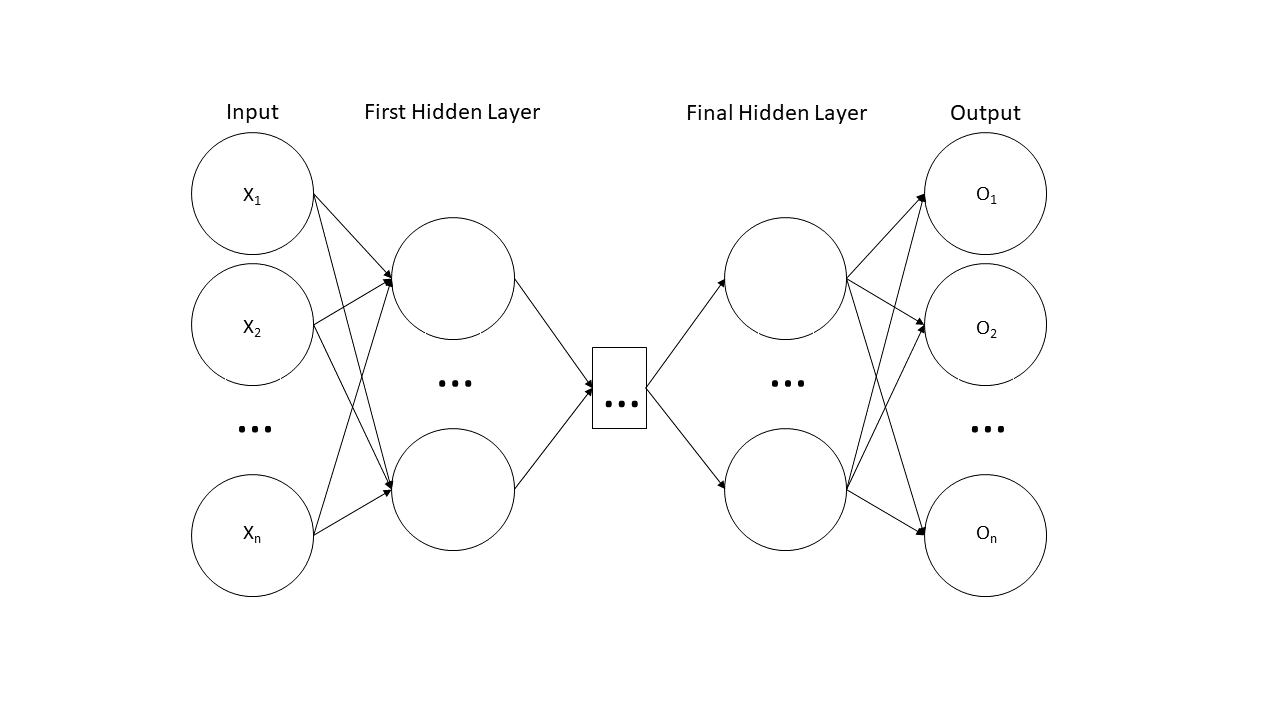
\includegraphics[width=1.0\textwidth]{figures/NN.png}
    \caption{Neural Network}
    \label{fig:NN}
    Diagram of a vanilla neural network
\end{figure}
It is important to note that in practice, the neural net actually approximates the argmin, as the optimization problem is typically not convex. 
\subsection{Training a Neural Network}
The actual training of a neural network is typically handled by whatever package one is creating their network in (in this case, Tensorflow), however we feel a brief overview would be helpful for some readers. We've previously introduced the idea that a neural network attempts to minimize the difference between the target and the output. One can then formulate the loss of the system on its training set as a function of the weights of the network. Then, one calculates the gradient of the loss function with respect to the weights. Finally, the weights are altered in the direction of greatest decrease of loss. This process is called gradient descent. 
\subsection{Backwards Propagation}
The actual calculation of a neural networks gradient of the loss function is typically performed automatically using whatever package the network is built in. This is done via an extended use of the chain rule. First, the network is run forward, the output is calculated, and intermediary values of the network are calculated. In the case of our vanilla network, we track the values $a_1 = W_1x + b_1$, and $a_i = W_i\sigma(a_{i-1})+b_i$ for $i\in\{2,...,n_l\}$. Then, the cost is \[C = \frac{1}{2}||\sigma(a_{n_l})-y||^2\] We calculate the first gradient \[\nabla_{a_{n_l}} C = \Big(\sigma(a_{n_l})-y\Big)\odot\sigma'(a_{n_l})\] and iteratively calculate the rest using chain rule. \[\frac{\partial C}{\partial{a_i^j}}= \sum_k\frac{\partial C}{\partial a_{i+1}^k}\frac{\partial  a_{i+1}^k}{\partial{a_i^j}}\] \[\frac{\partial  a_{i+1}^k}{\partial{a_i^j}} = (W_i)_{kj} \sigma'(a_i^j)\] 
This allows the final gradient calculations \[\frac{\partial C}{\partial (W_i)_{kj}} = \frac{\partial C}{\partial a_i^j}\sigma(a_{i-1}^j)\]
 \[\frac{\partial C}{\partial (b_i)_{j}} = \frac{\partial C}{\partial a_i^j}\]
 The actual calculations of backwards propagation do vary if the network structure is different, but follows the same general structure of featuring a forward pass followed by use of the chain rule.
\subsection{Recurrent Neural Networks }The recurrent neural network introduces a twist on the neural network structure, in the form of memory. The network's input is both the original input $x_k$, as well as the previous output of the network $o_{k-1}$.
\begin{figure}
    \centering
    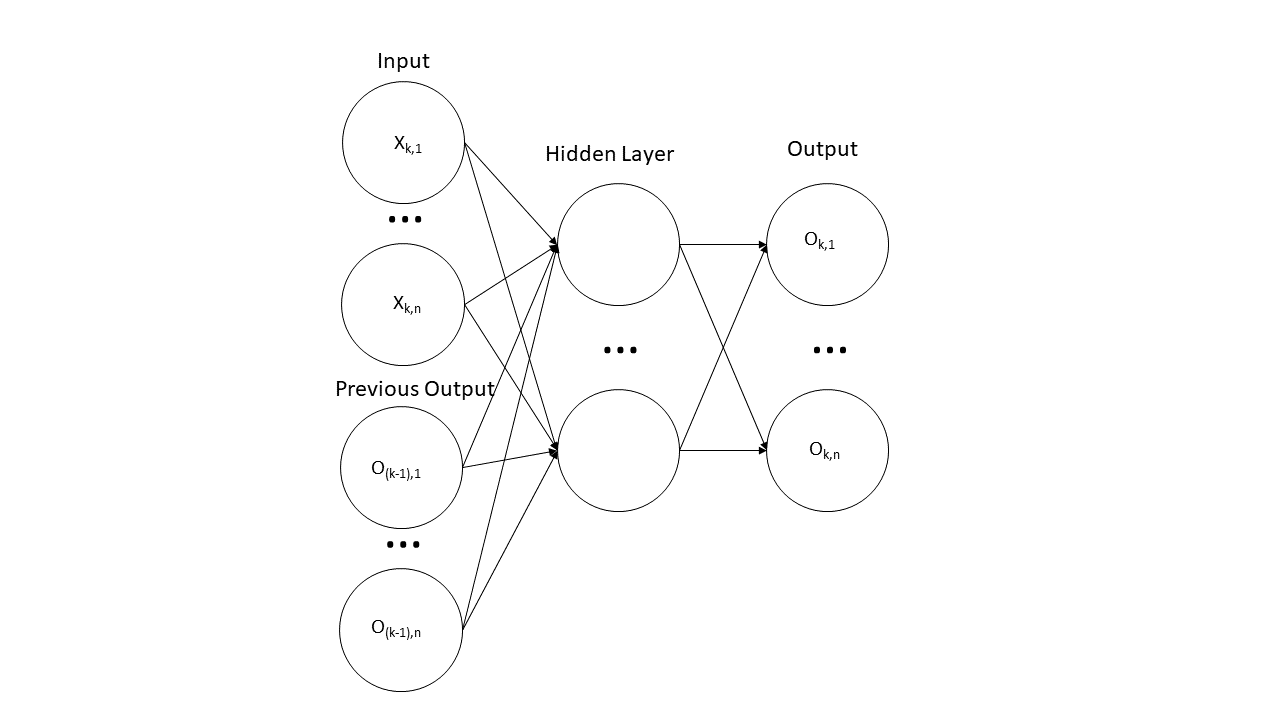
\includegraphics[width=1.0\textwidth]{figures/RNN.png}
    \caption{Recurrent Neural Network}
    \label{fig:rnn}
    Diagram of a vanilla recurrent neural network
\end{figure}
\subsubsection{LSTM}
The LSTM is one of the most ubiquitous RNNs in practice. The LSTM is a variant on RNNs that include a key difference to the vanilla RNN in its introduction of a specific memory cell. While the vanilla RNN has a method of passing information to the next state, its memory is restricted to its output, which inherently restricts the network's ability to maintain long-term memory. The vanilla LSTM accomplishes this by taking as input the current input $x_k$, the previous output, $o_{k-1}$, and the previous memory $h_{k-1}$. At the start of the cell calculation, we set \[z_k = [x_k,o_{k-1}]\] as a concatenation of the input and previous output. Next we calculate the forget gate,\[f_k = \text{sigmoid}(W^f z_k + b^f)\]This gate determines the amount of previous memory passing through to the next step. We then calculate what our memory update will be, as well as gate how much of that memory will be added to the memory cell.
\[g_k = \text{sigmoid}(W^g z_k + b^g)\]
\[ \hat{h}_k = \tanh(W^h z_k =b^h)\]
These are used to update the memory cell.
\[ h_k =  h_{k-1} \odot f_k + \hat{h}_k \odot g_k\]
Finally, the output is calculated with our new memory trace.
\[o_k = \text{sigmoid}(W^oz_k + b^o) \odot \tanh(h_k)\]
The LSTM's introduction of memory traces allows for long term dependencies to develop. It allows for much more robust pattern identification, and has become almost synonymous with recurrent nets due in large part to the success it has achieved. Still, we believe that there is room for better implementation of temporal data within the framework of a recurrent net than simply another input fed into an LSTM. Memory decay should be more explicitly tied to the temporal data, otherwise a burst of events in short time has the potential to quickly decay the memory of cells. For an excellent blog post describing the functionality and computation behind the LSTM network, see http://colah.github.io/posts/2015-08-Understanding-LSTMs/ \cite{LSTM-Blog}.